\section{The Two Hands of God}


\begin{quotex}
God brought the universe into existence as a Visible world and an Unseen world so that we might know the Hidden by the Unseen and the Manifest by the Visible. He described Himself with pleasure and wrath, and so He brought the world into existence as a place of fear and hope so we fear His wrath and hope for His pleasure. He described Himself with majesty and beauty, so He brought the universe into existence with awe and intimacy. It is the same for all that is connected with Him, may He be exalted, and by which He calls Himself. He designates these pairs of attributes by the two hands which He held out in the creation of the Perfect Man. 
\flright{\textsc{Ibn Arabi}, \emph{The Wisdom of Adam}}
\end{quotex}



\begin{wrapfigure}{rt}{.3\textwidth}
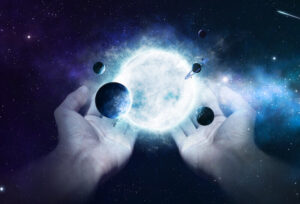
\includegraphics[width=.3\textwidth]{two-hands-of-God-300x204.jpg}
\end{wrapfigure}

Visible world includes the conditions of Manifestation: form and matter, space and time, life or consciousness. All the forms of things are ideas in the Divine Mind. Matter is pure possibility since matter cannot change unless acted upon by an outside force. In terms of physics, the totality of the possibilities of manifestation, i.e., the ``universe'', is like a universal Schrodinger's cat: it is neither dead nor alive until infused with form. That is vertical causation.

Since mathematics is the divided line between the unmanifest and the manifest, this can be understood by set theory. The things of the world are sets of certain ideas. Since there cannot be an actual infinity, the things of the world are always countable. However, in the unmanifest Divine Mind, which includes all possibilities of manifestation, there are increasingly higher and higher levels of order.

In our time bound state, we can only experience the order of the universe as an unfolding in space and time. That is why we usually miss the significance of events and things in the flow of time. As
\textbf{Rene Guenon} explains in \emph{Symbolism of the Cross}, everything happens out of necessity and according to higher principles. For example, he writes:

\begin{quotex}
the laws of a lower domain can always be taken to symbolize realities of a higher order, wherein resides their own profoundest cause; which is at once their principle and their end.
\end{quotex}


By the \textbf{Law of Correspondence}, everything in the world derives from, and therefore also expresses, a higher metaphysical principle. So the world is the expression of ever higher principles. Ultimately, all of manifestation is the expression of the complete idea in the divine Mind, from the beginning of the world until the end of time. At every instant, then, God is forming the world from the ideas and matter. One can develop the vision to see that the entire cosmos is a theophany, the manifestation of God's Will in space and time. The world is thus in God's hands, Divine Providence is active everywhere, even during what seems to be the darkest hours and times of tribulation.

Just as there is no set of all ordered sets, God is beyond Being and Time. He remains Unseen since we cannot now him in his Essence, such as we are.

\paragraph{The Perfect Man}


God created man as the perfect state of individual manifestation. The animals have as gross body and the subtle states of sensing and feeling. The angels lack sensory apparatus, so they cannot experience manifestation through the senses. Moreover, they do not have access to all of God's Names and Attributes, but just those appropriate to them.

However, man has the thinking functions in addition to the gross and subtle states of the animals. Unlike the angels, he has in potential the ability to understand God's Names. Ibn Arabi expresses it like this:

\begin{quotex}
God is your mirror in which you see yourself, and you are His mirror in which He sees His Names. His Names are not other than Himself.
\flright{\textsc{Ibn Arabi}, \emph{The Wisdom of Seth}}
\end{quotex}


Everyone comes into the world with a defined essence which includes talents and other qualities. There are no accidents, so even the time and place of our births are necessary. But essence is insufficient. Our task is to actualize our possibilities, based upon our essential features and the opportunities that present themselves.

To some, that may seem unjust, although God is not unjust. Our specific accomplishments in the world are individualized and cannot, and should not, be compared to others.

\paragraph{Hope and Fear}


God brings us blessings but He also brings us tribulations. They each require a different response. We need to feel gratitude for the good time, but patience and acceptance for the bad times. On the contrary, we usually take the good times for granted, as if they are normative rather than the exception.

In times of tribulations, the temptation is to recite platitudes similar to this: ``all things work for the good.'' Another response is a cynical pessimism common to the cultured sophistication of shallow men. Rather, tribulations warn us not to take comfort in the things and pleasures of the world; nor should we be embittered by the world.

Soren Kierkegaard develops this theme in the \emph{Edifying Discourses}. He says that obedience to God is the one thing needful. That requires faith in God's authority over the world and in His Providence.


\flrightit{Posted on 2021-05-06 by Cologero}

\begin{center}* * *\end{center}

\begin{footnotesize}
\begin{sffamily}

\texttt{Auld Wat on 2021-05-07 at 17:37 said:}

God has created me to do Him some definite service. He has committed some work to me which He has not committed to another. I have my mission. I may never know it in this life, but I shall be told it in the next. I am a link in a chain, a bond of connection between persons. He has not created me for naught. I shall do good; I shall do His work. I shall be an angel of peace, a preacher of truth in my own place, while not intending it if I do but keep His commandments. Therefore, I will trust Him, whatever I am, I can never be thrown away. If I am in sickness, my sickness may serve Him, in perplexity, my perplexity may serve Him. If I am in sorrow, my sorrow may serve Him. He does nothing in vain. He knows what He is about. He may take away my friends. He may throw me among strangers. He may make me feel desolate, make my spirits sink, hide my future from me. Still, He knows what He is about.
\flright{Saint John Henry Newman}


\hfill

\texttt{Angolmois on 2021-05-13 at 03:08 said:}

What about theodicy, as if the Absolute would not contain also evil? I can't understand how someone could portray God as ``wholly Good'' etc. as if God wouldn't be above the questions of good and evil which belong to the order of created beings. The greatest theological error of the Abrahamic faiths springing from Mazdaism has been to posit two insoluble principles -- one wholly good, one wholly evil -- as the foundation of ``monotheism''. Satan is nothing but the other face / hand of God, who also brings tribulations, as in Job.

\hfill

\end{sffamily}
\end{footnotesize}

